\documentclass[a4wide,10pt]{article}

\usepackage[dvips]{graphics,color}

\title{Word Sense Disambiguation Using English-German Parallel Corpora}
\author{Claire Taylor and Charlotte Wilson}
\date{1 November 2003}

\begin{document}
\maketitle

\section{Introduction}
Many supervised Word Sense Disambiguation (WSD) methods require
large sense-tagged corpus on which to train.
In the absence of already existing, reliable and accurate 
sense-disambiguation systems the generation of this sense-tagged text 
must be done by hand. As a result, sufficiently large corpora of 
sense-annotated training data for WSD are uncommon and very time-intensive 
to produce. This problem is refered to as the Knowledge Aquisition 
Bottleneck and is a major factor hindering the progress of WSD research.

An alternative approach to generating sense-tagged corpora makes use of 
differing sense distinctions between languages and uses parallel texts 
(one text in multiple languages) to sense-tag words in one language with 
their translations in the other. 

This approach has gained exposure due to the availability of a number 
of parallel corpora, especially on the web. Parallel corpora (one text 
in multiple languages) are reasonably common and are produced by a 
number of multilingual orgranisations and entities. For example  
the Canadian Hansard corpus is a French-English parallel text of 
the Canadian parliament and similarly the European Union parliamentary 
proceedings are documented as parallel texts in a number of European 
languages.  

Additionally, the use of parallel corpora generates a sense inventory that 
is readily applicable to Machine Translation and cross language Information 
Retrieval tasks \cite{yarowsky}.
The sense distinctions will correspond to translation 
differences in the parallel corpus and will be limited to the set of senses 
that are made in either of the langauges. In such applications full sense 
disambiguation will be unnecessary to tranlsate between the languages.    

For WSD tasks required for non cross-language specific applications, 
parallel polysemy across languages (and in particular closely related 
languages) may reduce the effectiveness of a sense-tagging system based on
word correspondences in parallel texts. In this case it may be more 
effective to use parallel corpora in languages that are not closely related 
and have had little contact historically (e.g. English and Chinese). Such 
languages can be assumed to share only a limited amount 
of sense ambiguity. In the case of more theoretical WSD research and in 
particular one-word WSD (as opposed to the all-words task), it may 
suffice to select words to disambiguate that are known to 
translate differently according to the sense in which they are used.

In our project we used English-German parallel corpora to generate 
sense-tags for an English word. Our aim was to make 
use of word correspondences in the English-German parallel text 
to disambiguate English words based on their German translations. We chose 
a limited set of English words that we knew translated as different
German words depending upon the sense they were used in. These words
were also used in the hand-annotated senseval corpus, which provided us with
a gold-standard against which to test our method.      

Our training data consisted of English-German parallel corpora, both of 
which had been preprocessed to be machine-readable and one-to-one 
sentence aligned. The first was de-news, a corpus consisting of 9,756 German 
radio news items human translated into English. 
However, despite its size of over a million words, this corpus contained only 
a limited number of instances of the ambiguous words. To address this problem,
we also used a second larger English-German parallel corpus - the Europarl 
corpus\cite{europarl}. This corpus is a collection of transcripts of the 
European parliamentary proceedings from 1996 to 2000 and contains roughly 20
milion words. For more information about the respective corpora see: 
\texttt{www.isi.edu/{\char'176}koehn/publications/de-news/} and 
\texttt{www.isi.edu/{\char'176}koehn/publications/europarl/}. 

Our approach to disambiguating an English word translated into various 
sense-distinct German words is summarized below.    

\begin{enumerate}
\item 
\begin{enumerate}
\item Train the translation module to generate sense tags according
to the German translation of the ambiguous English word. 
\item Sense-tag the English section of the parallel corpus, generating training 
data for WSD. 
\end{enumerate}

\item Train the WSD module on the sense-tagged training corpus.
\item Test the WSD module against a portion of the senseval corpus.
\end{enumerate}

\section{The Translation Module}

The translation module generates an appropriate sense-tag for our ambiguous 
word based on its translation in the parallel text.  
Sense-tag generation is a two stage process in which the  
translation module first identifies the translation of our ambiguous
word in a given sentence of the parallel corpus and then groups the 
resulting translations into sense groups. This second step is only neccessary 
in the case that the translations themselves do not adequately or 
consistently correspond to a ``sense'' (e.g. if compound word forms or 
complex morphology commonly occur as part of the translations and 
pre-processing such as stemming in the translation language is not possible).


\subsection{Identifying Word Correspondences in Parallel Texts}

The parallel corpora which we used have been pre-processed to be one-to-one 
sentence aligned using an algorithm by Church and Gale \cite{gale91program}. 
The next step in the translation process is identifying the correspondences 
between the words in the parallel texts. For example, given the aligned 
sentences below, identifying which word in the German sentence is the 
translation of the English word {\bf \em interest}:

\begin{quote}
The government is already paying DM225 million in daily {\bf \em interest}.

Schon jetzt zahle der Bund jeden Tag 225 Mio. DM Zinsen. 
\end{quote}

\noindent With no knowledge of German, the choice is fairly arbitrary, 
and could be any German word in the sentence (although admittedly 
the currency figures can probably be discounted). 

There are a number of possible approaches which we could have taken to 
this problem. The first would be to get possible translations as user input, 
however this strategy requires the user to have a reasonable knowledge of 
both languages of the parallel text. Even limited only to German and English -
the pair of languages used in our project - this constraint would certainly 
prevent many users from being able to run the system. Furthermore, it is
likely that a system for English WSD using parallel corpora may utilise 
parallel corpora in other languages. The requirement that the user have 
knowledge of all and any such languages would further restrict system 
usability.

Another approach taken by many systems that manipulate parallel corpora 
is to make use of machine-readable bilingual dictionaries. 
Whilst such resources are becoming more common and easier to obtain, we
were unable to find a freely available German-English machine-readable 
dictionary. Aside from this problem of availability, it is quite likely that 
dictionary entries cannot encompass the breadth of variety in actual usage 
of the language (e.g. idioms and compound-nouns).

Both of the above-metioned approaches make the assumption that there exists 
a fixed set of ``senses'' for sense-ambiguous word that are 
able to be listed (either by the user or by a lexicographer). There has been 
some debate about what a ``sense'' actually is \cite{manning99}
and what granularity of sense inventory is appropriate in 
WSD. The granularity of the sense inventory used will influence the resulting 
sense-tags on the training data used for the disambiguation method. Therefore
generating the sense-tags from the corpus itself gives a reasonably
accurate sense inventory for the training text.  

Our approach was to use statistical methods trained on large
parallel corpora to identify the word correspondences. 
We began with a naive method that was based on maximizing a simple 
co-occurence frequency count for the ambiguous word and its possible 
translations. Rather unsurprisingly, the results for this method were 
consistently poor. The translation produced for all our ambiguous words
was {\it der} or {\it die} (German for {\it the}).   
Another approach we implemented was to use Mutual Information to score 
possible translations (as described by Church and Gale \cite{gale91word}). 
However 
this approach allocated the same ranking to a large number of German words 
that co-occur in sentences with the ambiguous word and failed to 
distinguish between them: ``Mutual information picks up the fact that there 
are strong associations ... . Unfortunately it is not very good at 
deciding which association is stronger.''\cite{gale91word}

Another possible approach which we did not implement is to use the EM 
Algorithm \cite{brown}. However, Church and Gale are critical of 
this approach for two reasons. The first is that it is resource hungry and
as a result the size of the voacbulary used may need to be limited and the 
second is that this method may not be robust and can get stuck at a local 
maxima of the probability of the observed pairs.

The method we choose is based on one described by 
Church and Gale \cite{gale91word}. 
This method assigns a score to every possible translation of the ambiguous
word. That is, a score is calculated for every word which occurs in a German
sentence that is aligned with an English sentence containing the ambiguous 
word. The score is based on a contingency table constructed from the counts 
of the number of sentences containing the words as folows:

\begin{center}
\begin{tabular}{|c|c|c|}
\hline
				& = {\it Zins} 	& $\neq$ {\it Zins}
\\ \hline
= interest			& 5 		&  156
\\ \hline
$\neq$ interest			& 2 		& 68518 
\\ \hline
\end{tabular}
\end{center}

Church and Gale describe how the table can be computed: 

\begin{tabular}{rl} 
cell a ({\it upper-left})  &= freq({\it interest, Zins})
\\
cell b ({\it upper-right}) &= freq({\it interest}) - freq({\it interest, Zins})
\\
cell c ({\it lower-left})  &= freq({\it Zins}) - freq({\it interest, Zins})
\\
cell d ({\it lower-left})  &= N - a - b - c
\\
\end{tabular} 

where N is the total number of aligned sentences 

The score for each pair of words is calculated using:
\begin{center}
$\phi$$^2$ = $\frac{(ad - bc)^2}{(a + b)(a + c)(b + d)(c + d)}$
\end{center}

This formula is in fact a variation of the $\chi$$^2$ formula for a 
two-by-two contingency table. $\chi$$^2$ is a measure used to estimate the 
dependence between two co-occuring words and is used to test for 
dependence (i.e. whether the words coocur more often than chance). 
$\chi$$^2$ compares the observed frequencies with the frequencies 
expected for independence (chance cooccurence). If the difference between 
the observed and expected frequencies is large then we reject the null 
hypothesis of independence. This measure is also commonly used to idenitify 
collocations within the one language \cite{manning99}
and is calculated using:
\begin{center}
$\chi$$^2$ = $\frac{N(ad - bc)^2}{(a + b)(a + c)(b + d)(c + d)}$
\end{center}
\noindent The constant N provides an additional measure of the significance 
of the co-occurence in the corpus. However, this is not necessary when 
looking at possible translation pairs as we know that such a pair must exist in 
the aligned sentences.     

After calculating the $\phi$$^2$ score for every possible translation of the
ambiguous word, a tranlsation for a particular English word is found by 
taking the most likely translation (i.e. the translation with the 
highest $\phi$$^2$ score) that occurs in the corresponding German sentence. 
For example, if we were trying to disambiguate {\it interest} in the English 
sentence:  
\begin{quote}
The conditions would be as good as never before , no hint of 
{\bf \em interest} increases, excellent figures for such companies as Krupp 
, BASF and BMW , and a low inflation rate .
\end{quote}

\noindent we first calculate a list of possible tranlsations ranked by 
$\phi$$^2$ score: 

\begin{quote}
['Interesse', 'Zinsen', 'Zinsbesteuerung', 'Zins', 'Zinssenkungen', 
'Zinseinkuenfte', 'Zinspolitik', 'Zinsniveaus', 'Zinsniveau', 
'Zinserhoehungen',{\bf \em 'Zinserhoehung'}, 'Zinseinkuenften', 
'Eigeninteresse', 'Desinteresse', 'Abgeltungssteuer', 'Leitzinsen', 
'Bundesbank', 'zurueckerstattet', 'zinslosen', 'zinsguenstigen', ...]
\end{quote}

\noindent and then look in the aligned German sentence, taking the highest 
ranking possible tranlsation to be the correct translation. 

\begin{quote}
Die Rahmenbedingungen dafuer seien so gut wie nie , keine Spur 
von {\bf \em Zinserhoehung} , vorzuegliche Unternehmenszahlen von Firmen 
wie Krupp , BASF und BMW und eine geringe Inflationsrate .
\end{quote}

\noindent The resulting translation is {\it Zinserhoehung}. 

The statistical translation algorithm based on $\phi$$^2$ results in a 
reasonably accurate list of possible translations. For example, the English 
word {\it interest} is commonly translated as either {\it Interesse} and 
{\it Zins}. The ranked list of translations by $\phi$$^2$ score we get after
training on the de-news corpus is: 

\begin{quote}
[(0.1096, 'Interesse'), (0.1065, 'Zinsen'), 
(0.0319, 'Zinsbesteuerung'), (0.0221, 'Zins'), 
(0.0186, 'Zinssenkungen'), 
(0.0186, 'Zinseinkuenfte'), (0.0124, 'Zinspolitik'),
(0.0124, 'Zinsniveaus'), (0.0124, 'Zinsniveau'), 
(0.0124, 'Zinserhoehungen'), 
(0.0124, 'Zinserhoehung'), 
(0.0124, 'Zinseinkuenften'), 
(0.0124, 'Eigeninteresse'), 
(0.0124, 'Desinteresse'), 
(0.0124, 'Abgeltungssteuer'), 
(0.0111, 'Leitzinsen'), 
(0.0078, 'Bundesbank'), 
(0.0062, 'zurueckerstattet'), 
(0.0062, 'zinslosen'), 
(0.0062, 'zinsguenstigen'), ...]
\end{quote}

\noindent From this list it is clear that the most probable translations 
include both the root forms of the two most common translations as well as 
a number of compounds and inflected forms including the root forms.    

In practice we do also get translations of {\it interest} as 
{\it 5,5} or {\it Bundesbank}. A solution to this would 
be to set a threshold value for $\phi$$^2$ (as per the $\chi$$^2$ test) under
which we give a null translation. We have not implemented this threshold 
as the second step of the sense-tag generation process, sense-grouping the
translations, allows the user to specify the number of sense-tags that 
are generated.

\subsection{Classifying the Translations into Sense Groups}

From the example list of possible translations above, it is clear that 
the direct German translation of the ambiguous word may differ within senses. 
For example the financial sense of {\it interest} - translated as {\it Zins} -
may include direct translations such as {\it Zinsniveau} or {\it Leitzinsen}.
These words are examples of the infamous ability in the German language to 
compound numerous words together and form one long compound noun. The 
direct German translation is therefore, not necessarily a good sense-tag.

The ideal solution to this problem would be to run a stemmer over the German 
text before translating, removing morphological endings and splitting 
compounds. As a result of this pre-processing the direct German translations 
would be an uninflected root form and would more consitently give accurate 
indications of senses. However, we have not been able either to access such a 
stemmer or develop one (that is outside the scope of this project).    

Instead, to address this problem, we have used a (rather unsophisticated)
algorithm that aims to group the direct translations into approximate sense 
groups. This algorithm is based on the idea that we can locate the 
root form of the sense group by searching for common substrings within the
translations. That is, we aim to classify the tranlsations according to 
common morphology. 

Classification is performed only on the top ranked possible translations 
(we take the top 30 in our implementation) in order to get only the
most likely common forms. We take a four letter prefix from each translation
and search for this string as a substring of the remaining translations. 
Then we group together all translations with a common substring and 
re-calculate the $\phi$$^2$ score for the group. This new score can then 
be used to rank the sense groups, as we did the translations from most to least
likely.    
 
From these sense groups we require only the more likely as sense-tags. 
Whilst one possible approach would be to take only those senses with a 
$\phi$$^2$ score above a certain threshold, we found that an appropriate 
threshold value was difficult to set and a value that was appropriate for 
one ambiguous word might not be appropriate for another. Therefore, instead 
of setting a threshold, we take the top n most likely senses. Of course, the
number of possible senses may vary for each word and some translations may 
not be grouped together or ranked highly enough by this algorithm and thus, 
the number of required senses is a system parameter that can be specified 
by the the user.       

This algroithm does have some drawbacks and will not perform as well as 
pre-processing the text to remove inflection and split compounds. For example,
if the common morpheme occurs word finally in all the compounds that are 
translations it will never be found. This would be the case for
words such as {\it Politik} (German for {\it politics}) which commonly occurs 
at the end of German compunds such as {\it Medienpolitik} or 
{\it Frauenpolitik}. Additionally, a four letter prefix may contain 
German prefixes such as {\it -un} or {\it -ab} (or both together 
{\it -unab}!). Grouping words according to these prefixes will result in
unreliable and somewhat random sense groups. In cases such as this a longer 
prefix may be more effective, however this may mean that short common  
morphemes are not identified.   


\section{WSD Methods}
Even though we decided to tackle the problem of word sense disambiguation
using a bilingual corpus, there are many learning methods we could have
implemented.
Due to time constraints it was impossible to implement as many as we would
have liked and instead we have implemented three simple classifiers:  A base
case that assigns the most frequent sense to every occurrence of the ambiguous
word, a simple Naive Bayes classifier that uses Bayes theorem to classify each
occurrence, and a bagger that combines multiple Naive Bayes classifiers.
We decided to implement these methods instead of other possible ones as
Naive Bayes is a relatively straigthforward method to implement that 
performs reasonably
well and we can compare the results of one classifier to the results that
we get when we use the bagging method.
Each of the methods was implemented using a separate class that contained
a train() function and a sense\_tag() function.
The following sections outline the different methods mentioned above.

\subsection{A Base Case}
In order to have a base line to compare our word sense disambiguator we
implemented a base case model.
For this the training phase consists of counting the number of times each
sense appears and then assigning the most common sense to every occurrence
of the ambiguous word during the testing phase.
This method is not very ``intelligent'' but does give us a base line that 
we can aim to beat with other learning methods.


\subsection{Bayesian Learning}
        A Bayesian classifier is a statistical classifier based on Bayes                Theorem.  The algorithm makes that assumption that all features are
        equally important and are independent of one another.
        In the case of word sense disambiguation this equates to the words
        either side of the ambiguous word, i.e. all the words in a given
        context window, being treated as equally important. This means that if
        we take a context window of five words either side, a word immediately
        before the ambiguous word has as much impact on the predicted sense
        as a word five words before it.


        Bayes Theorem, upon which our classifier is based, is as follows:\\
        \begin{center}
        $ P(H|E) = \frac{P(E|H)P(H)} {P(E)} $\\
        \end{center}
        where H is a hypothesis, E is the evidence.\\
        In the case of our project the hypothesis is a possible sense of the
        word we are disambiguating and the evidence is the words in a given
        context window around this word.

 Now suppose we let $E = [E_1, E_2, \ldots, E_n]$ then \\
        \begin{center}
        $P(H|E) = \frac{P(E_1|H)P(E_2|H)...P(E_n|H)P(H)}{P(E)}$\\
        \end{center}
        In the case of our classifier each of the $E_i$'s corresponds
        to a word in the context window.
        So when we encounter a word in testing that was not seen
        with this sense in training $P(word|sense) = 0$ and so
        $P(H|E) = 0$.


        To overcome this problem we implemented smoothing
        to give the unseen events a small probability and accordingly 
	adjusted the
        probabilities of those events that were seen during training.
        The smoothing method chosen was Witten-Bell's equations which are
        as follows:\\
        \begin{center}
        $p_i^* = \frac{c_i} {N + T} $ if $c_i > 0$\\
        \vspace{0.5cm}

        and\\
        \vspace{0.5cm}

        $p_i^* = \frac{T}{Z(N + T)} $ if $c_i = 0$\\

        \vspace{0.5cm}
        \end{center}
        where N is the total number of word tokens seen in training,\\
        T is the number of word tokens seen with this sense\\
        and Z is the number of words with a zero count.


        \subsubsection{Bagging}
        When people make critical decisions they often take into account the
        opinions of experts instead of relying on their own judgement.
        So why should word sense disambiguation be any different?
        Bagging, which stands for Bootstrap Aggregation, is the simplest way
        of combining the predictions made by several models.  Each model makes
        a {\it vote} on the classification of the test data which in
        our case is the sense of the ambiguous word.


        Bagging attempts to overcome the problem of a limited training data
        set by replacing selected instances in the training data with replicas
        of other training instances.
        A number of different models are trained on these different, but
        not independent, data sets.  In testing each model is used to
        predict the sense of each occurence of the ambiguous word with
        the most frequently
        predicted sense becoming the assigned sense.

\subsection{k-means Clustering}
We initially implemented k-means clustering but decided to remove it from the
system for two reasons.  Firstly, it performed very badly, clustering all
occurrences of the ambiguous word as the one sense, and secondly because we
changed the interface of all classifier modules to take the training data
as a list of SenseLabeledText instances instead of the original TaggedTokens.
This meant that we would have to re-write this class even though we knew it
performed badly if we were to include it in the final system.  After some
discussion we decided we would not re-write k-means and so it has not been
included in the final system.


\section{Evaluating Performance}

To evaluate the performance of our system we report the precision, recall
and f measures of every sense that is predicted for the test data as well as
the overall accuracy.

Precision, recall and f-measure are defined as follows:\\
\begin{center}
$ \mbox{precision} = \frac{\mbox{number retrieved that are relevant}}
                                {\mbox{total number retrieved}}$
\\
\vspace{5mm}

$ \mbox{recall} = \frac{\mbox{number relevant that are retrieved}}
                        {\mbox{total number relevant}}$
\\
\vspace{5mm}


$ \mbox{F-measure} = \frac{1} { \frac{\alpha} {precision} + \frac{1-\alpha} {recall}} $\\
\vspace{5mm}
\end{center}
where $0 \leq \alpha \leq 1$

For this project we interpreted this to be:\\
\begin{center}
$ \mbox{precision} =$\\
\vspace{5mm}
 $\frac{\mbox{No of times a word is tagged as this sense and it is the correct sense}}  {\mbox{total no of times our system tagged a word as this sense}}$\\
\vspace{1cm}

$ \mbox{recall} =$ \\
\vspace{5mm}
$\frac{\mbox{No if times a word is tagged as this sense and it is the correct sense}} {\mbox{total no of times this sense appears in the test data}}$\\
\end{center}
With these definitions of precision, recall and f-measure it is possible to
evaluate the performance of our system.


\subsection{Aligning Senses For Evaluation}
One of the problems associated with word sense disambiguation using bilingual
corpora is how to evaluate performance.
If a word sense disambiguator is trained and tested on the same corpus
then it is trivial to compare the sense tags of the original text with
the sense tags the word sense disambiguator has predicted.  However, in the
case where the training and testing data do not come from the same source,
as is the case with this project, it is necessary to decide which assigned
sense tag corresponds to which test data sense tag.

One the method that could be used to match sense tags with the assigned tags
would be to take each assigned sense in turn (from the most frequent
to the least frequent) and calculate the
f-measure if this sense was to correspond to each senses in the test data.
The assigned sense and the test sense with the highest f-measure are considered
the same sense when calculating precision and recall.
When this is run on the results of a Naive Bayes classifier with a context
window of 3 after being trained on a portion of the Senseval corpus we found
that the assigned senses and the original senses matched up perfectly even
though the Naive Bayes model did not predict every sense correctly.
However this was not always the case when matching up the German sense tags with
the Senseval senses.

\subsection{Exploring the Problem}
In order to make our system as flexible as possible we have implemented the
word sense disambiguation methods in such a way that certain parameters can
be changed to allow the user to fully explore the problem domain.
For example, for the Naive Bayes model it is possible to specify the
size of the context window that is to be used for both testing and training.
In bagging it is possible to specify the number of models you wish to use
and also the number of training data examples you wish to remove before
training.

\section{Results}
\label{results}
As we can not be sure that the German translation of the ambiguous word
corresponds to the sense of the particular occurrence, the results of the
word sense disambiguation may not be great.  In order to evaluate the
performance of the classifier independently of the translations
we trained the classifier on a portion of the Senseval text.
We ran the classifier on each of the words and recorded the f measures
for each sense as well as the base case.  This test was run several times
and the average f-measure was taken as the final result.
\subsection{Naive Bayes}
\label{res_naivebayes}
The following graph shows the f-measure values for the senses
of the word interest when tagged using a Naive Bayes classifier.
\begin{center}
\Large{Results: Senseval Training Data}
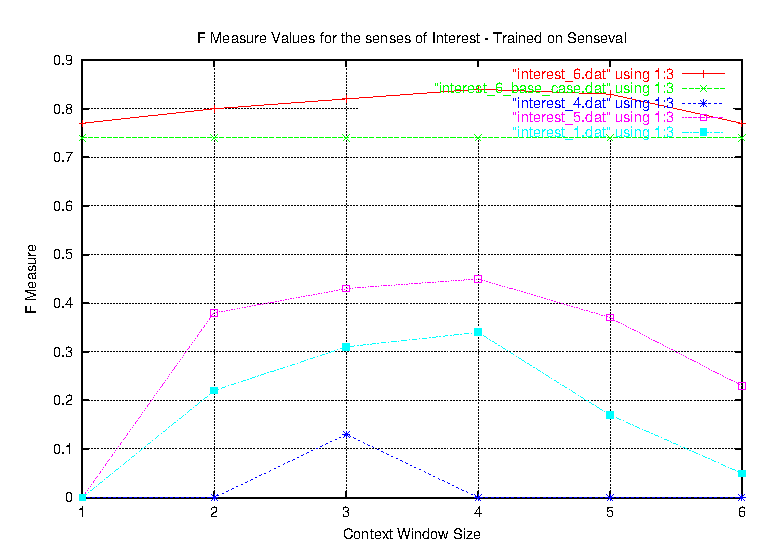
\includegraphics{interest_nb.eps}
\end{center}

With this as a guideline as to how our system performs on properly sense
tagged data we could realistically examine the results when it is run on
a bilingual corpus.
The following graph shows the f-measure values for the senses of the word
interest when run on the de-news corpus.

\begin{center}
\Large{Results: De-news Training Data}
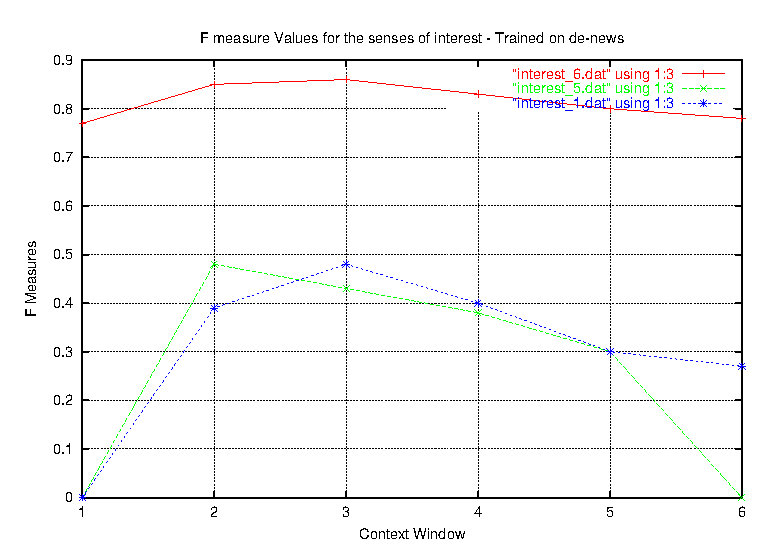
\includegraphics{interest_nb_de.eps}
\end{center}

\subsection{Bagger}
Despite the bagger classifier having multiple models to help decide which
sense to assign to an ambiguous word,  it did not add much to the accuracy
of the system.

When run using Senseval as training data for a Naive Bayes classifier
with a context window of 3, the sense interest\_6 achieved an f-measure
of 0.82.  When we used a bagger to sense tag the data (also trained on
Senseval) we got the following results for sense interest\_6 summarised 
in the table below:\\
\begin{center}
\begin{tabular}{|l|r|r|r|}
\hline
Replacement & t = 5 & t = 10 & t = 15\\
\hline\hline
50 & 0.79 & 0.82 & 0.81\\
\hline
100 & 0.86 & 0.85 & 0.84\\
\hline
\end{tabular}
\end{center}
We also ran the same tests using the de-news corpus as the training data
and got the following results with the German sense 'zins' being mapped to
interest\_6:\\
\begin{center}
\begin{tabular}{|l|r|r|r|}
\hline
Replacement & t = 5 & t = 10 & t = 15\\
\hline\hline
50 & 0.79 & 0.82  & 0.85 \\
\hline
100 & 0.80  & 0.75 & 0.78\\
\hline
\end{tabular}
\end{center}




\section{Discussion}
After some initial test cases we discovered that the results were very skewed
when we trained the classifiers on the Senseval data.
For some words we would get 100\% precision,  for others we would get 0\%.
Upon analysing the training and test data we discovered that the senses in
Senseval seemed to be grouped together, i.e. The instances of the sense
HARD1 mostly seemed to appear together.  This meant that the classifiers were
being asked to classify an instance of the ambiguous word where it had never
seen the correct sense in training and so would never get it correct.
To overcome this problem we introduced some shuffling of the data before it was
separated into separate test and train sets.
This solved the problem and we began to get meaningful results.
\subsection{Base case}
In certain cases, testing the base case provided some odd results.
From the definition of recall and the knowledge of how the
base case classifier works, one would expect recall for all base case runs to be
100\%.  However, on most runs of the base case on the ambiguous words line or
serve recall hovered around the 96 to 97\% mark instead of achieving the
expected 100\%.  Careful inspection of the data revealed that the cause of this
was that Senseval treated {\it serve}, {\it servingi} and {\it served} as forms
of the same word, {\it serve}, and hence sense-tagged all three forms.  The
same applies to {\it line} where the form {\it lines} is treated the same.  
This resulted
in differing counts for the senses as our classifiers only look for an
exact match with the ambiguous word rather than looking for words that
are based on it.  As this problem does not have a large effect on the
accuracy measures of the program we decided not to try to fix it but
decided to document it instead.  A more accurate classifier would be one that
checks to see if a word can be stemmed to the original ambiguous word in order
to decide if it needs to be disambiguated.

\subsection{Naive Bayes}
From the graph of Senseval results
in \S~\ref{res_naivebayes} we see that the base case result when
run and tested using Senseval is approximately 74\%.
When using the bilingual corpus to train the word sense disambiguator
we got an F-measure of 74\% for the sense 'inte' which mapped to the
Senseval sense 'interest\_6' for the context window of 4.
The sense 'zins' is also tagged for some instances but receives an f-measure of
0\%.
So by using a bilingual corpora for word sense disambiguation we managed
to equal the base case using a Naive Bayes method.

Although it is disappointing that we did not manage to beat the base case,
it must be noted that by using a translation
module we have added a certain amount of error.  We can not be certain that
the word we decide is the German translation of the ambiguous word is in fact
the correct one, let alone be sure that the different translations of the
word correspond to the different sense-groupings in the test data.
So with this in mind the word sense disambiguator did reasonably good job
at performing the disambiguation, achieving results as good as
the base case.

We did attempt to run the system on the EuroParl corpus however the data is
some what skewed.  A frequency count of the senses for each of the instances
of the ambiguous word in the training data shows that the sense 'inte'
accounts for 82\% of the sense tags.  This results in a word sense disambiguator
that only performs as well as the base case, assigning everything to have
the sense 'inte'.
As a result of this we have not included any results from the EuroParl corpus
as we never found the classifier to tag using a sense other than 'inte'.

\subsection{Bagger}
As stated in the results section, the bagger added little improvement to
the performance of the naive bayes classifier.
However there are a few things to notice.
Notice how for a replacement value of 50 there is little improvement
 (and in some cases
a negative one!)  and for a replacement value of 100 there are small 
improvements for the t values of 5, 10 and 15 of 4, 3 and 2\% respectively.
Similar results were achieved for the other senses of interest but are not 
listed here as the data for interest\_6 gives a good indication of the 
performance of the bagger.
However, for the amount of extra computations that are required to get these 
results we only got a very small improvement.

It is also interesting to note that the bagger on the bilingual corpus performed
better than the bagger on Senseval for a replacement value of 50 and with 15
iterations.


\section{Conclusion}

The area of word sense disambiguation suffers from the
Knowledge Aquisition Bottleneck.  This results in the need to find
sources of data other than the typical hand annotated corpus.
A bilingual corpus offers a different approach to the problem.
Instead of training a disambiguator on sense tagged text, we can use 
the
property that for some languages, the translation of a word in English
may correspond to several different translations.

This project, using the German language and four ambiguous words,
illustrated
that although it is possible to use a bilingual corpora to perform
word sense disambiguation, the results are not as good as running the
same methods on typical sense labelled text.
Although the bilingual corpus approach did not compete with the
sense labelled text approach, we did find that it performed suprisingly
well in some cases equalling the base case of latter approach.

There are many factors that could be changed to help improve the
results of this system.  For example the bilingual corpora tended to be
skewed
to favour certain senses of the ambiguous words and hence the 
classifier
trained on that data also tends to favour those senses.
So finding a training corpus that represented each of the senses 
according
to
their natural distribution rather than heavily favouring one sense 
would improve the performance.
Another possible improvement to the system would be to use English
stemming and
part-of-speech tags to improve the performance of the naive Bayes classifier.

In conclusion, we found that the bilingual corpora approach to word 
sense
disambiguation is a promising approach that has many areas that could 
be adjusted to improve the overall performance of the system.


\section{Assessment Criteria} 

The HLT algorithms implemented in our system include $\phi$$^2$ scoring,
Naive Bayes, Bagging and classification by morphology. These algorithms are 
described in detail in the relevant sections above. 

The training data used included both hand-annoted sense-tagged text from the
Senseval corpus and the two English-German parallel corpora described above. 
The system creates sense-tagged text from the parallel corpora in the same 
format as that produced by the Senseval corpus reader in nltk. This enables
the user to compare system performance using the different corpora and 
evaluate the effectiveness of sense-tagging with translations in a 
parallel corpus.   

Additionally, the system has been implemented to enable the user to explore 
the performance of a various WSD methods with various parameter settings
(these are described fully in ``System Usage'' below).  Settings for both the
translation module (e.g. the number of senses) and the WSD modules (e.g. 
the size of the context window) can be varied allowing the user to explore the 
problem domain.  

The system has been designed with modules independent of one another, 
enabling problem-free development and future modifications to single
module. For example, it would be easy to ``plug-in'' a different translation 
module or WSD method. 

\section{System Usage Instructions}

\subsection{Paths to the Corpora}

\begin{itemize}
\item To run the system using the either of the parallel corpora
        you must ensure that the relevant path variables are set.
        These can be set at the top of the parallelCorpus module
        (parallelCorpus.py).  
\item To run the system using the senseval corpus (in nltk) ensure
        your NLTK\_CORPORA environment variable is set.
\end{itemize}

\subsection{Running the System}

\begin{enumerate}
\item Interactive Mode

        This is the default mode and is most user friendly as it validates
        user input. The system prompts the user interactively to
        enter values for the system parameters. To run the program in
        interactive mode type:

\begin{quote}
                 python senseDisambiguator.py
\end{quote}

\item Command-line Mode
        Input paramemters are not validated in this mode. System behaviour
        with invalid input may be user unfriendly.

        To run the program in command-line mode type with the default
        settings type:

\begin{quote}
                python senseDisambguator.py sense\_disambiguator
\end{quote}


        To run the program and override the defaults, you must enter values
        for all parameters (described below). Type:

\begin{quote}
                python senseDisambguator.py sense\_disambiguator [method
                        context\_window replacement iterate corpus num\_files
                        ambig\_word num\_senses]
\end{quote}

\end{enumerate}

\subsection{The Translation Module Demo}

The translation module is an important component of the system. Therefore
there are two demo methods for this module.

\begin{enumerate}
\item Given an English word and a German sentence, get the German
translation of the English word in the given sentence.

        To run this with the default parallel corpus and number of files type:
\begin{quote}
                python senseDisambiguator.py translate [english\_word
                        german\_sentence]
\end{quote}

        To run this, specifying the parallel training corpus and number
        of files type:
\begin{quote}
                python senseDisambiguator.py translate [english\_word
                        german\_sentence corpus num\_files]
\end{quote}


\item Given an English word get its 20 most likely German translations.

        To run this with the default parallel corpus and number of files type:
\begin{quote}
                python senseDisambiguator.py translate\_list [english\_word]
\end{quote}

        To run this, specifying the parallel training corpus and number
        of files type:
\begin{quote}
                python senseDisambiguator.py translate\_list [english\_word
                        corpus num\_files]
\end{quote}
\end{enumerate}


\subsection{Input Parameters and Defaults}

\begin{itemize} 
\item 
Default settings:	method=1, context\_window=3, replacement=50, 
iterate=10 corpus=3, num\_files=100, ambig\_word="interest", num\_senses=2 

\item 
method:			An integer between 1 and 3 (inclusive), where 1
               is naive bayes, 2 is naive bayes with bagging and 3
                is the basecase. See the report (report.pdf) in the
                assosciated documentation for more information on these
                WSD methods.

\item 
context\_window: A positive integer (including 0) or -1, specifying the size
                of the context window that naive bayes uses (i.e. the
                number of words either side of the ambiguous word). Entering
                -1 sets the context window to be the whole of the sentence
                in which the ambiguous word occurs. If running the basecase
                then this value should be set to 0 or None.

\item 
replacement:    The number of training instances that are to be replaced.
                This is used for bagging only.  Each of the models (total
                number of models trained is equal to the value in iterate -
                see below) has a different data set created from the training
                data set by replacing 'replacement' instances with copies of
                other training instances from the remaining data.  For
                more information on bagging see the report or inline
                documentation for the class.  If not running the bagger
                then this value should be set to 0 or None.

\item 
iterate:        The number of models that will be trained for bagging.
                Each of the models will be asked to predict the most likely
                sense during testing and then the most frequently predicted
                sense will be assigned.  If not running the bagger then this
                value should be set to 0 or None.

\item 
corpus:         An integer between 1 and 3 (inclusive), where 1 is the
                senseval corpus, 2 is the the de-news parallel corpus and 3
                is the europarl parallel corpus. See the report (report.pdf)
                in the assosciated documentation for more information on
                these corpora.

\item 
num\_files:     The number of files of the europarl corpus to use - an integer
                between 1 and 353 (inclusive). The europarl corpus is very
                large, therefore the user can specify how many of the 353
                files in the corpus to train on. If running the system with
                a different corpus this value should be set to 0 or None.

\item 
ambig\_word:    One of "interest", "hard", "line" or "serve". The ambiguous
                word to use (the system performs WSD on one word only).
                Enter the full word.

\item 
num\_senses:    The number of sense distinctions to make when training on one
                of the parallel corpora. For a language such as German
                with many compound nouns, possible translations are
                grouped into "senses" by common morphology. If using the
                system with a different language that does not have these
                compound constructions, set num\_senses to 0, to get the
                direct translation as a sense-tag. Naturally, in order to
                disambiguate with sense-groupings (i.e. in German) this
                should be set at 2 or more.

\end{itemize}

\subsection{Example Commands on the Command-Line}
\begin{itemize}

\item To run the Naive Bayes classifier with a context\_window of 2, on the 
first 50 files of the europarl corpus, disambiguating ``interest'' with 
2 senses, type: 
\begin{quote}
	python senseDisambguator.py sense\_disambiguator 1 2 0 0 3 50 interest 2
\end{quote}
\item To run the Naive Bayes classifier with Bagging with a context\_window 
of 5 and replacement of 20 for 10 iterations, on the de\_news corpus, 
disambiguating ``hard'' with 6 senses, type: 
\begin{quote}
	python senseDisambguator.py sense\_disambiguator 2 5 20 10 2 0 hard 6
\end{quote}
\item To run the basecase classifier on the senseval corpus, disambiguating 
``line'' type: 
\begin{quote}
	python senseDisambguator.py sense\_disambiguator 3 0 0 0 1 0 line 0
\end{quote}
\end{itemize}




\begin{thebibliography}{99}

\bibitem{brown} P.F. Brown  S. A. Della Pietra, V. J. Della Pietra, and 
R. L. Mercer (1993). ``The mathematics of statistical machine translation: 
Parameter estimation.'' {\it Computational linguistics}, 19, pp.263--312.

\bibitem{gale91program} William A. Gale and Kenneth Ward Church (1991). 
``A Program for Aligning Sentences in Bilingual Corpora''. {\it Meeting of the 
Association for Computational Linguistics}, pp. 177-184.

\bibitem{gale91word} William A. Gale and Kenneth Ward Church (1991),
``Identifying Word Correspondences in Parallel Texts''.{\it Proceedings of the
DARPA SNL Workshop}.

\bibitem{europarl} Phillip Koehn. ``Europarl: A Multilingual Corpus for 
Evaluation of Machine Translation''. Draft, Unpublished,

\bibitem{manning99} Christopher D. Manning and Hinrich Schutze (1999).
``Foundations of Statistical Natural Language Processing'', MIT Press.

\bibitem{yarowsky} Yarowsky, D (2000). ``Word Sense Disambiguation.'' 
In R. Dale, H. Moisl and H. Somers (eds.) The Handbook of Natural Language 
Processing.  New York: Marcel Dekker, pp. 629-654. 

\end{thebibliography}


\end{document}

